% Generated by benchmark.py
% Requires booktabs, graphicx, float in your preamble.

\begin{table}[H]
  \centering\small
  \setlength{\tabcolsep}{6pt}
  \caption{Models tested: model name, node count (before distribution), and preview.}
  \label{tab:rt-scene-overview}
  \begin{tabular}{@{}lrl@{}}
    \toprule
    \textbf{Model} & \textbf{Nodes} & \textbf{Preview} \\
    \midrule
    \texttt{01\_artemis} & 29 & 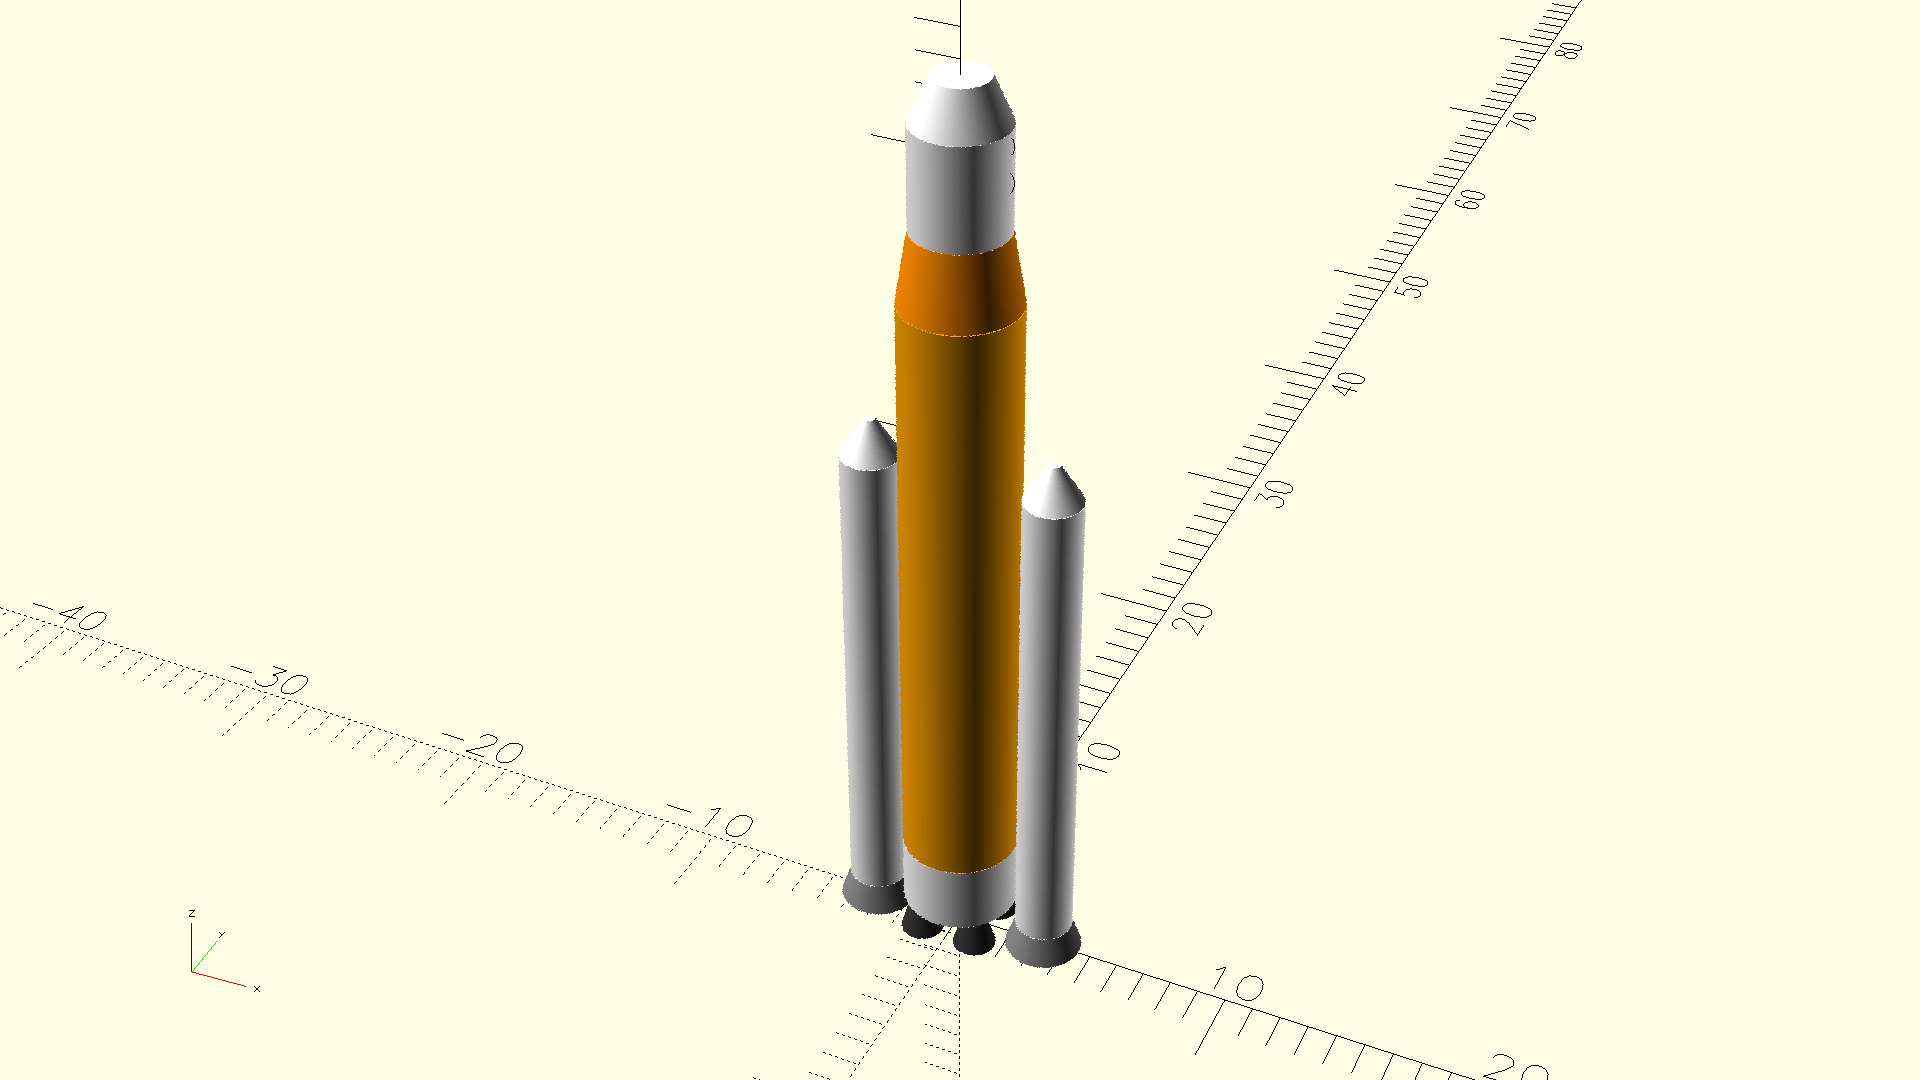
\includegraphics[height=2.8cm]{benchmark_results/01_artemis/frame.png} \\
    \texttt{02\_cheese} & 163 & 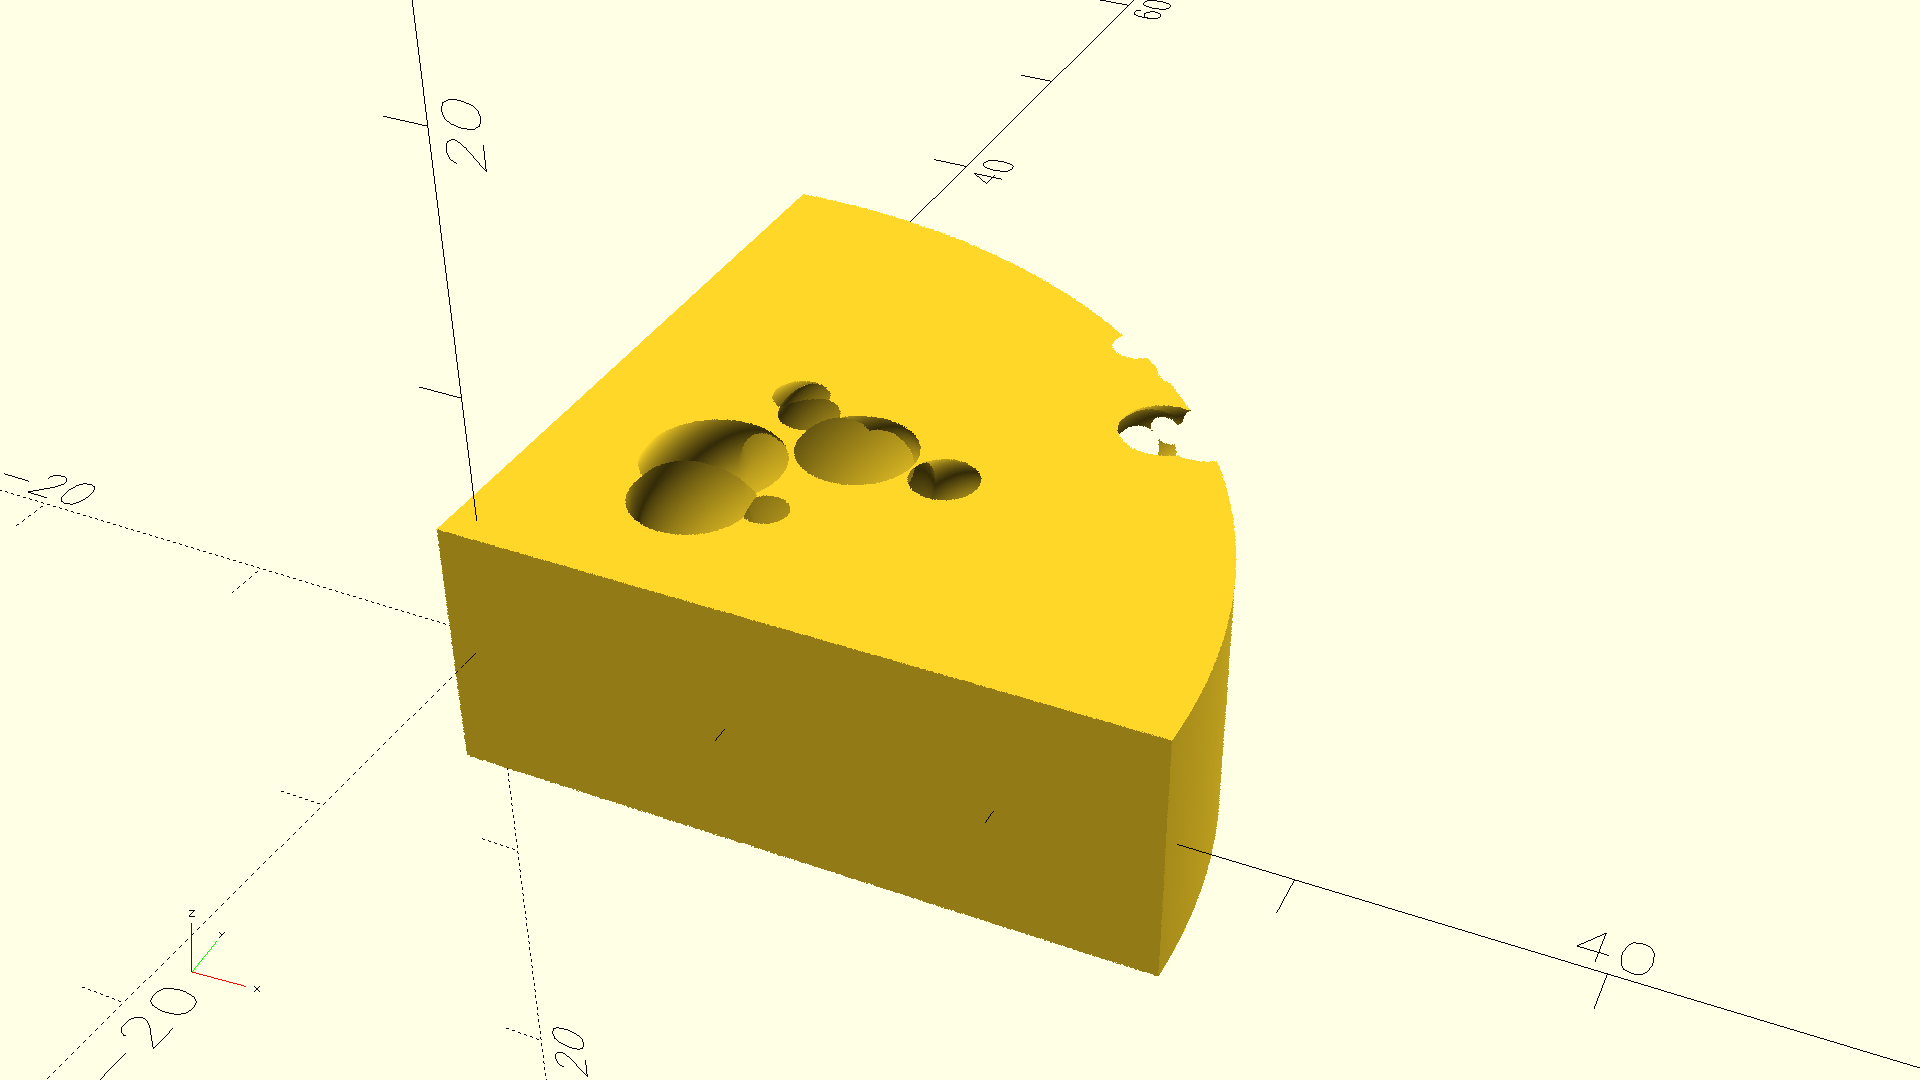
\includegraphics[height=2.8cm]{benchmark_results/02_cheese/frame.png} \\
    \texttt{03\_shuffled\_spheres} & 149 & 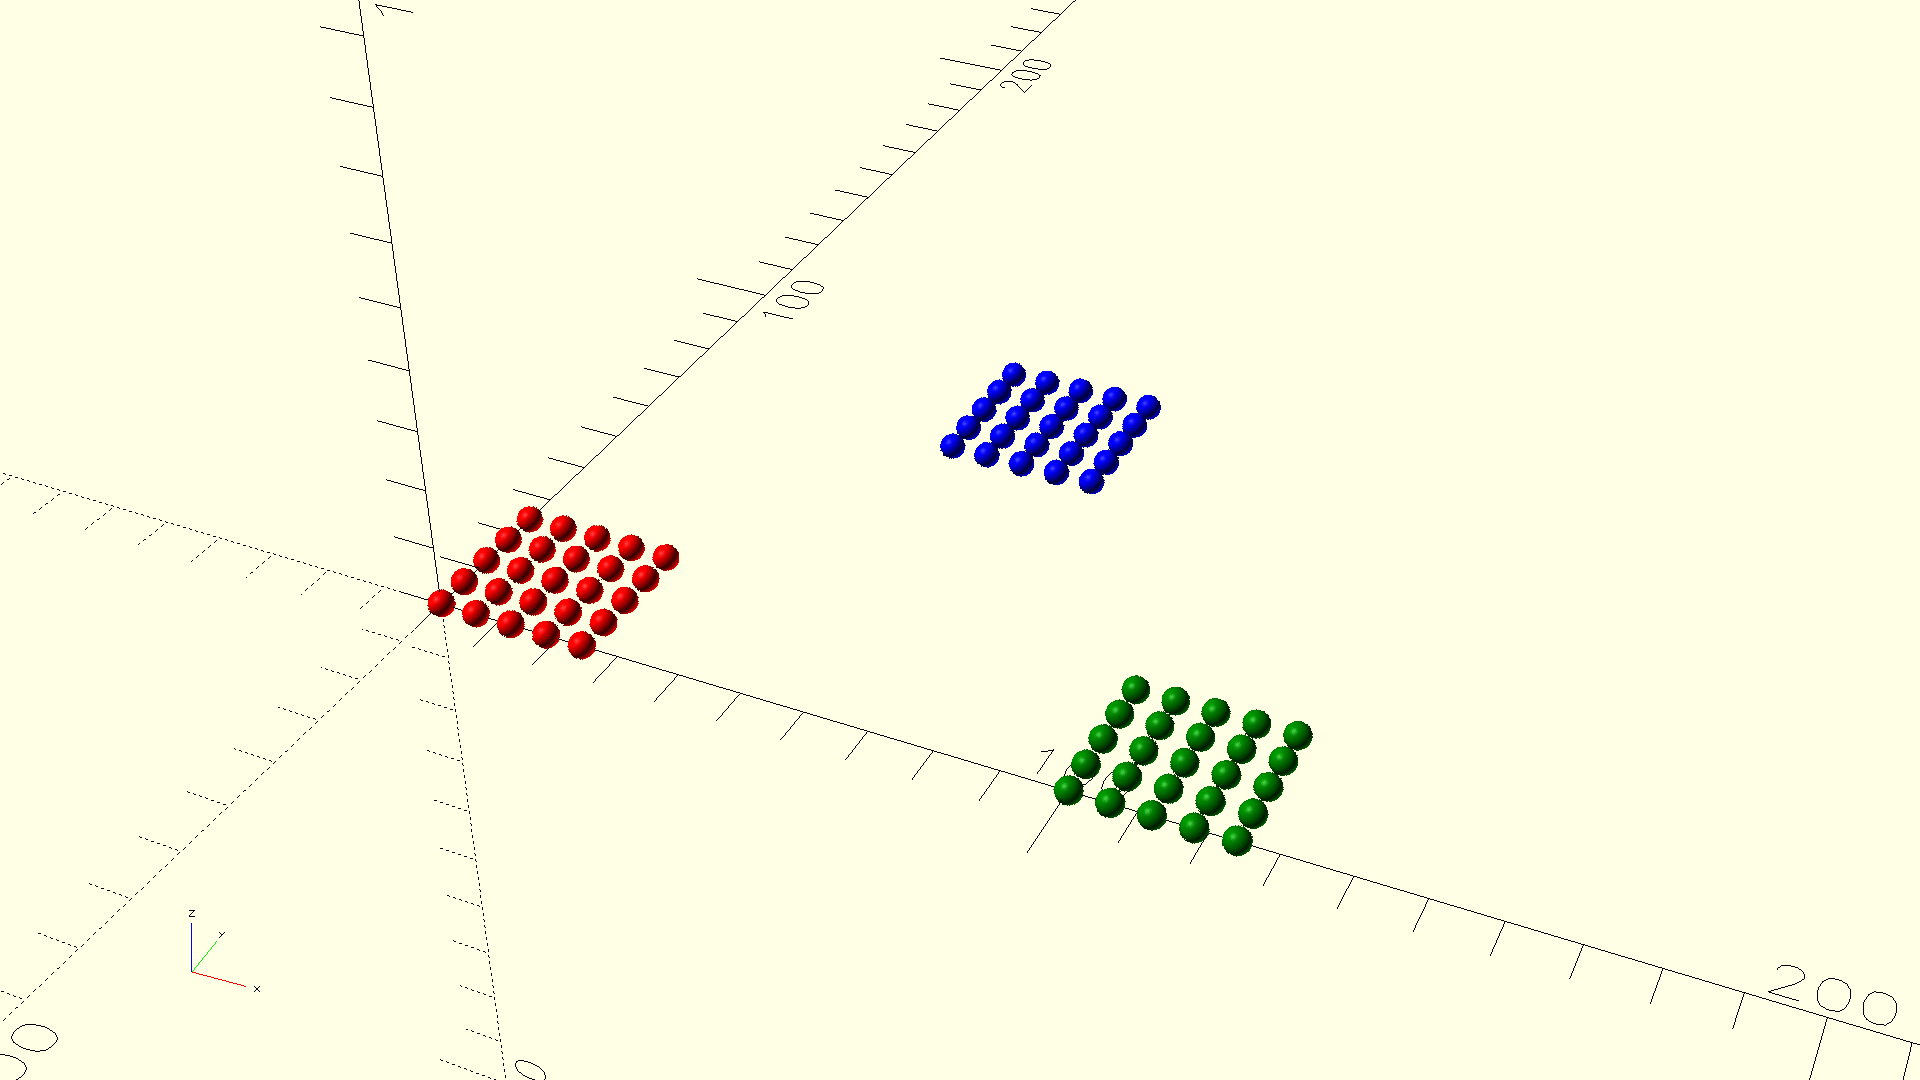
\includegraphics[height=2.8cm]{benchmark_results/03_shuffled_spheres/frame.png} \\
    \texttt{04\_distrib} & 389 & 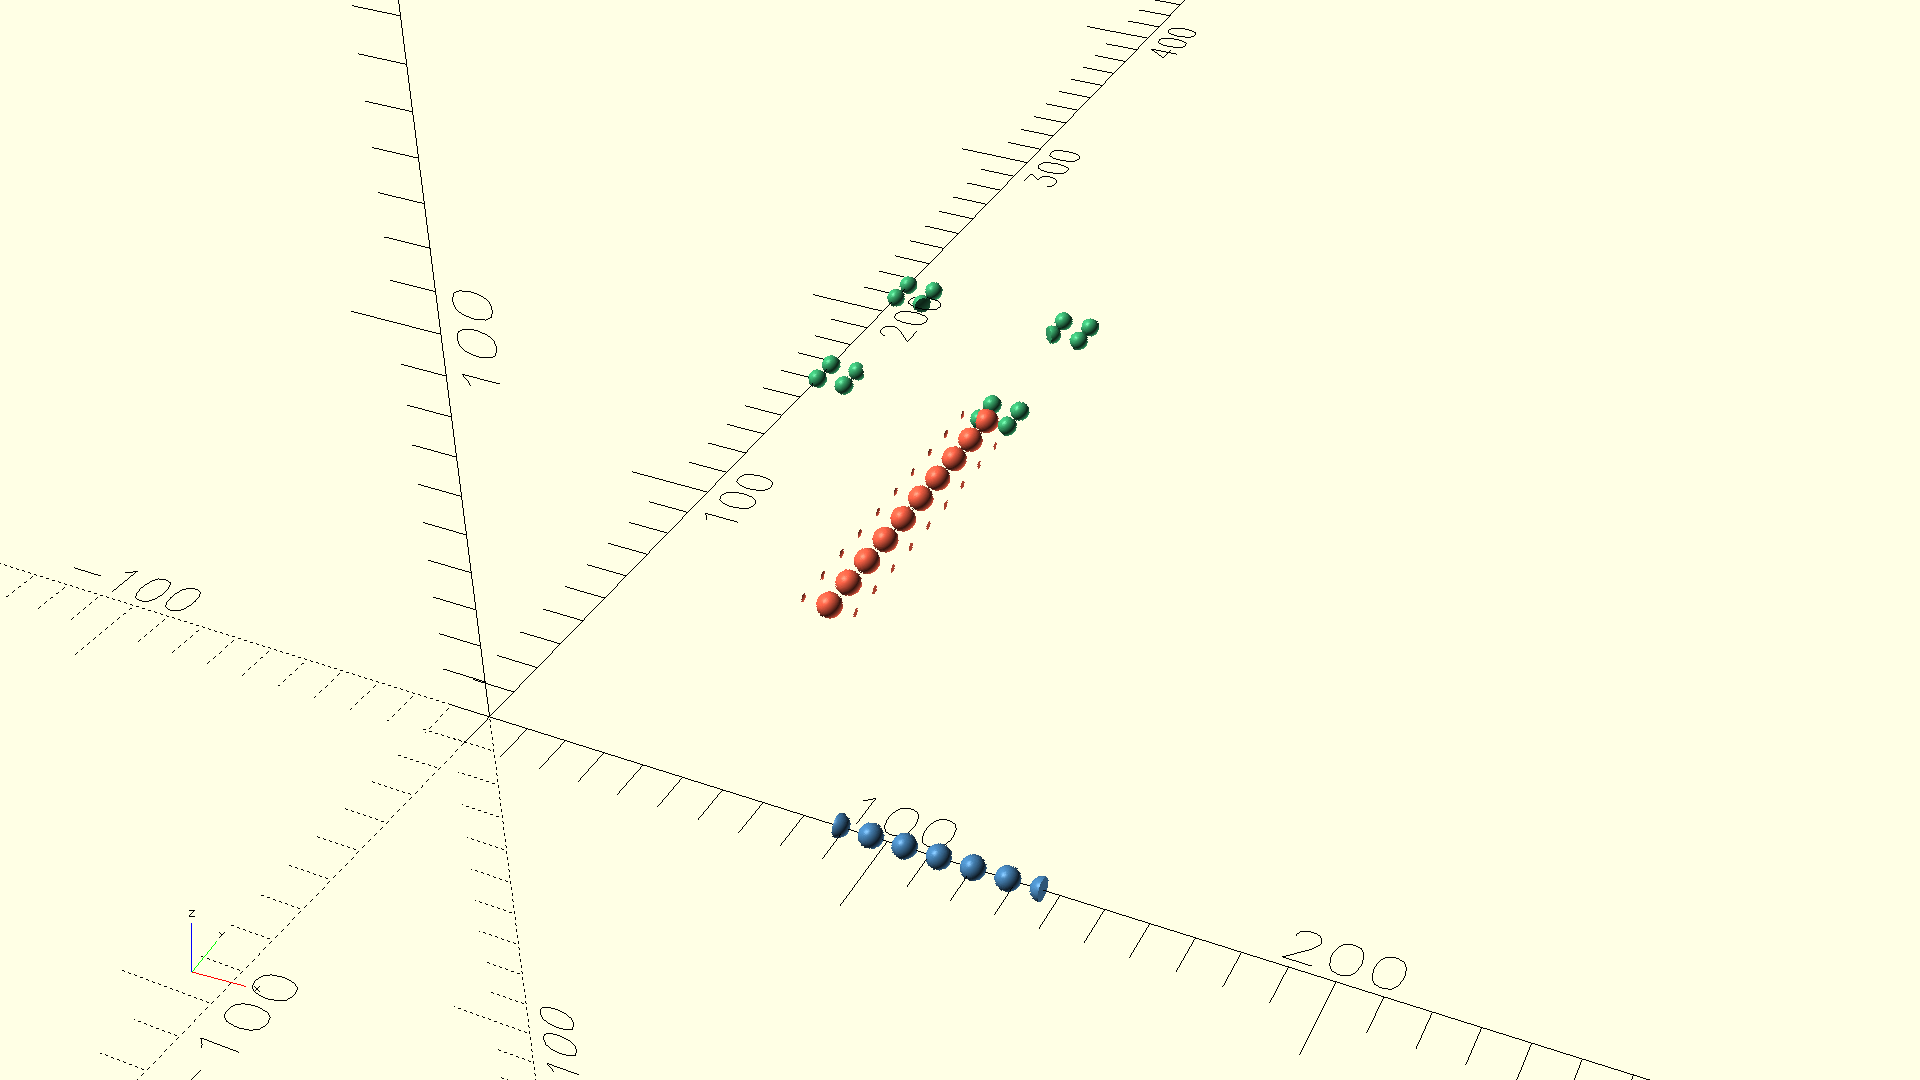
\includegraphics[height=2.8cm]{benchmark_results/04_distrib/frame.png} \\
    \texttt{05\_kd\_postdist} & 385 & 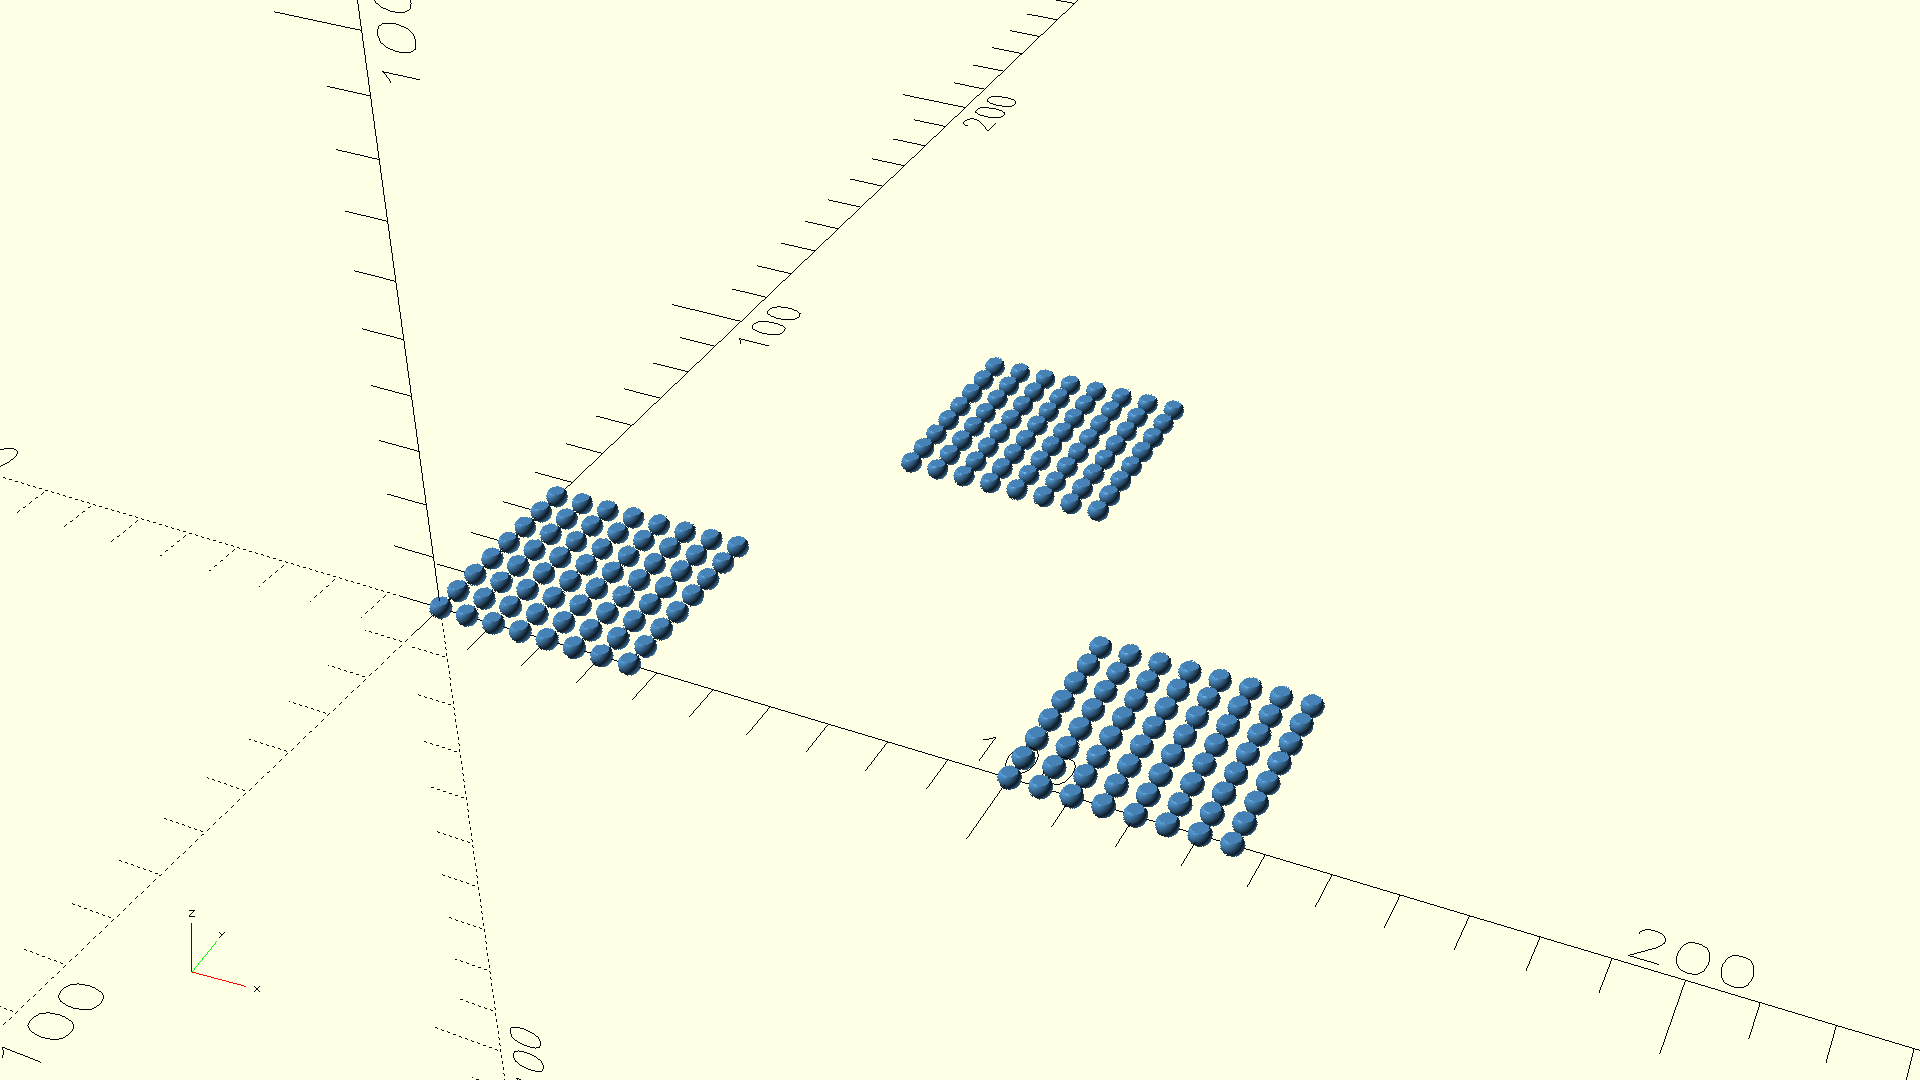
\includegraphics[height=2.8cm]{benchmark_results/05_kd_postdist/frame.png} \\
    \texttt{06\_sphere\_grid} & 1023 & 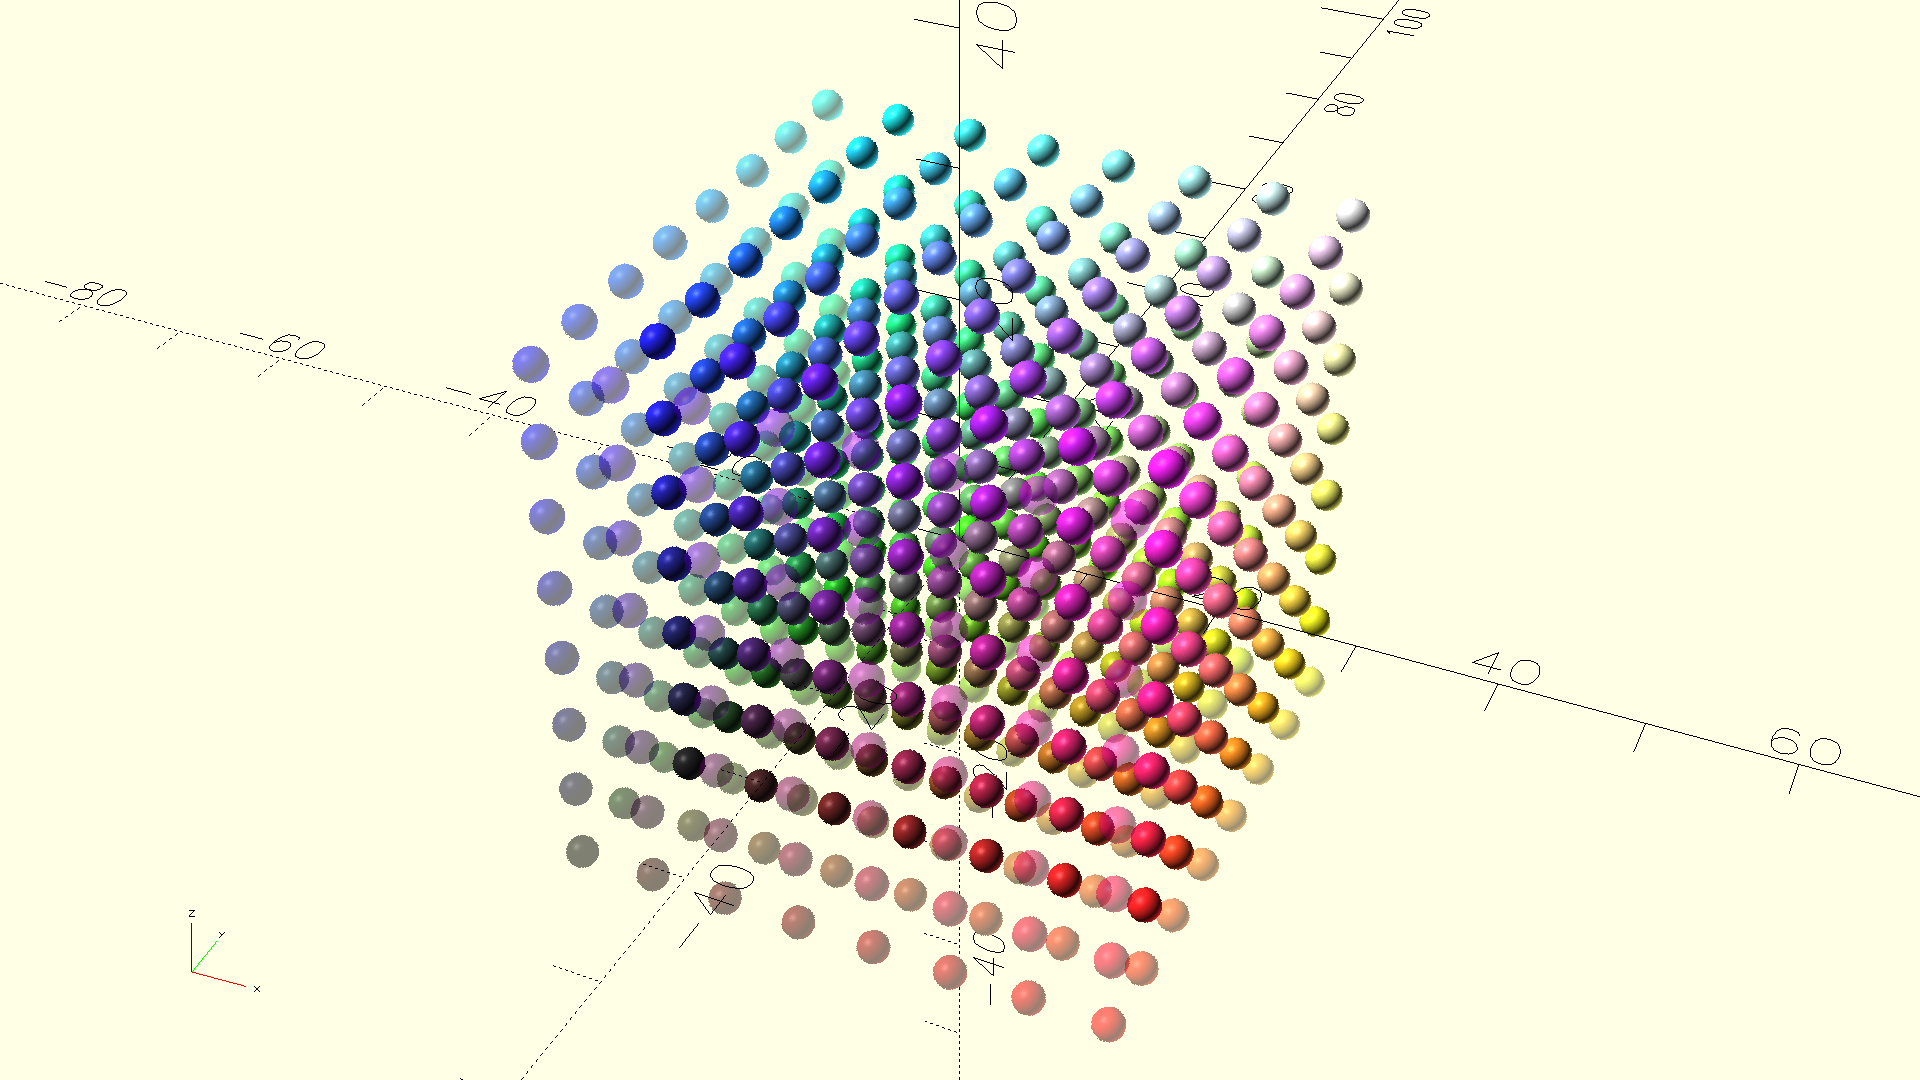
\includegraphics[height=2.8cm]{benchmark_results/06_sphere_grid/frame.png} \\
    \texttt{07\_artemis\_grid} & 1919 & 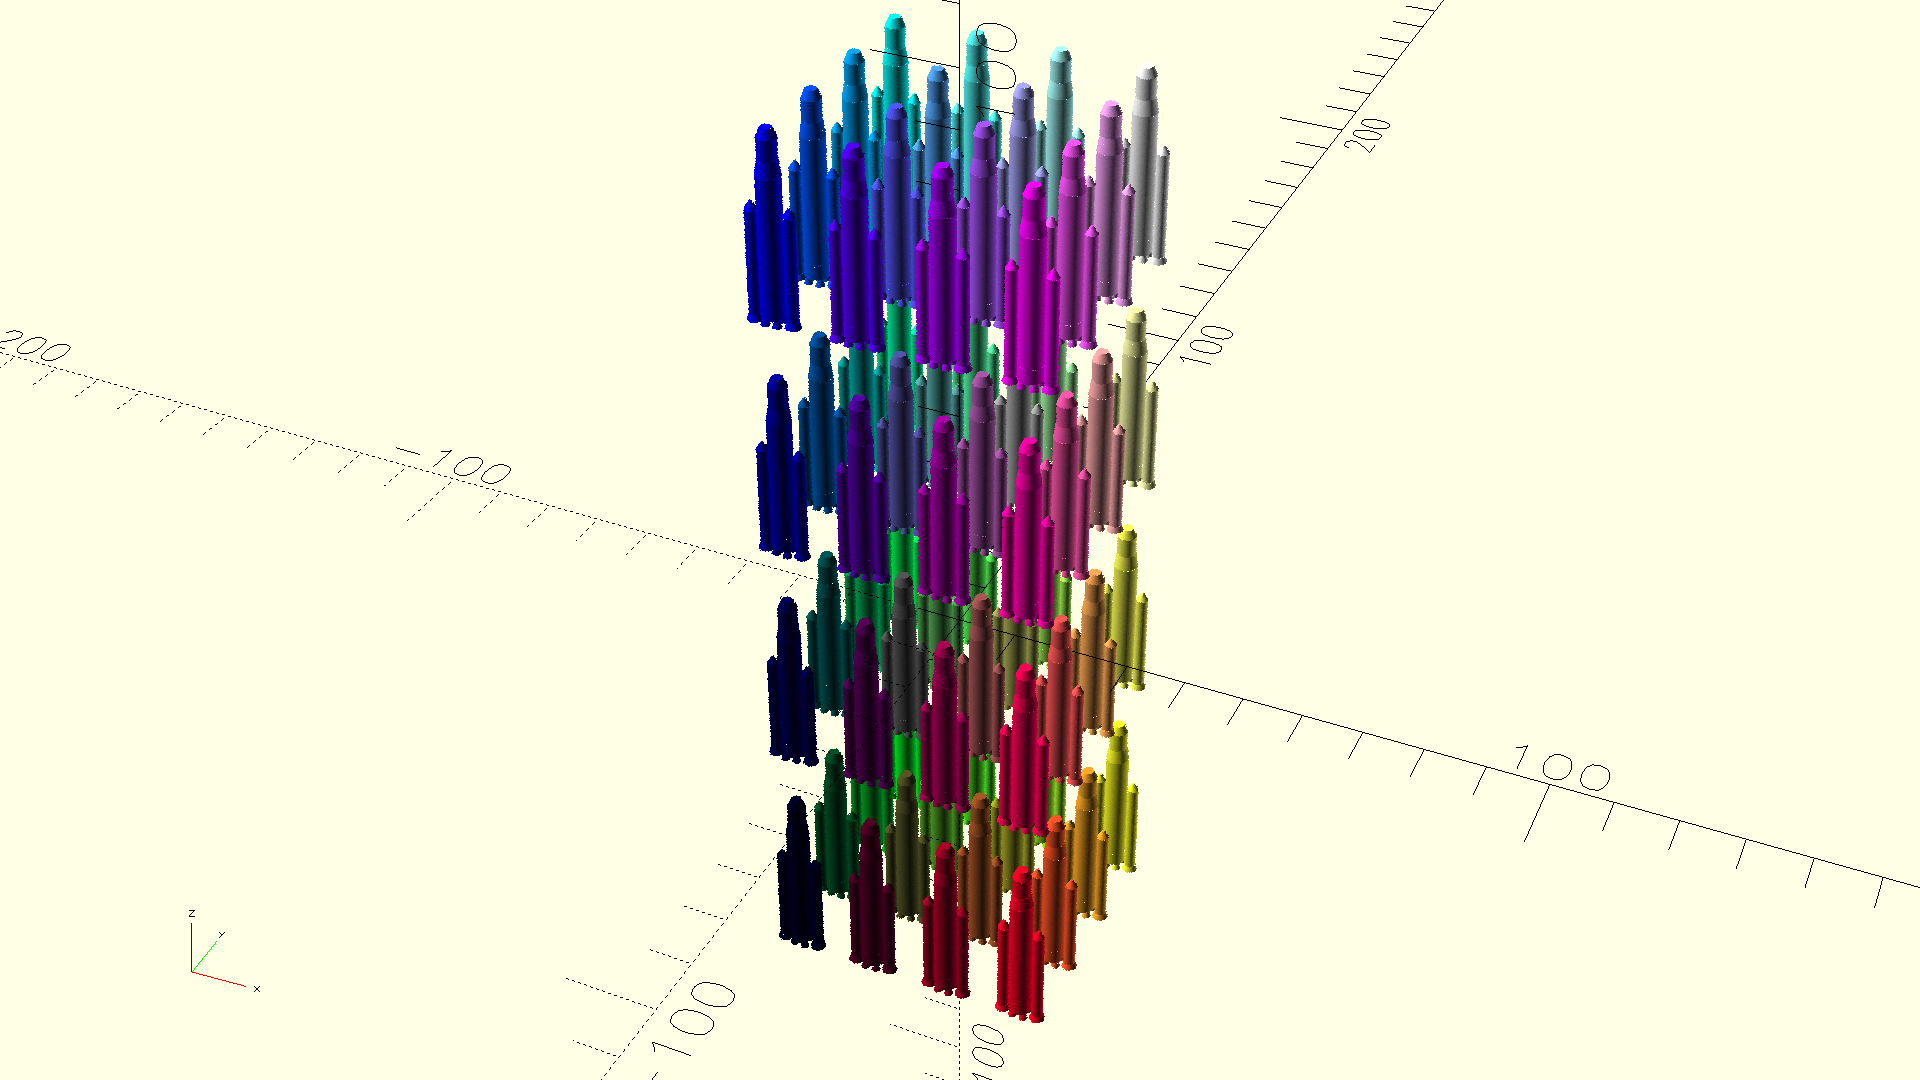
\includegraphics[height=2.8cm]{benchmark_results/07_artemis_grid/frame.png} \\
    \bottomrule
  \end{tabular}
\end{table}
